\documentclass[
  bibliography=totoc,     % Literatur im Inhaltsverzeichnis
  captions=tableheading,  % Tabellenüberschriften
  titlepage=firstiscover, % Titelseite ist Deckblatt
]{scrartcl}

% Paket float verbessern
\usepackage{scrhack}

% Warnung, falls nochmal kompiliert werden muss
\usepackage[aux]{rerunfilecheck}

% unverzichtbare Mathe-Befehle
\usepackage{amsmath}
% viele Mathe-Symbole
\usepackage{amssymb}
% Erweiterungen für amsmath
\usepackage{mathtools}

% Fonteinstellungen
\usepackage{fontspec}
% Latin Modern Fonts werden automatisch geladen
% Alternativ zum Beispiel:
%\setromanfont{Libertinus Serif}
%\setsansfont{Libertinus Sans}
%\setmonofont{Libertinus Mono}

% Wenn man andere Schriftarten gesetzt hat,
% sollte man das Seiten-Layout neu berechnen lassen
\recalctypearea{}

% deutsche Spracheinstellungen
\usepackage[main=ngerman]{babel}


\usepackage[
  math-style=ISO,    % ┐
  bold-style=ISO,    % │
  sans-style=italic, % │ ISO-Standard folgen
  nabla=upright,     % │
  partial=upright,   % ┘
  warnings-off={           % ┐
    mathtools-colon,       % │ unnötige Warnungen ausschalten
    mathtools-overbracket, % │
  },                       % ┘
]{unicode-math}

% traditionelle Fonts für Mathematik
\setmathfont{Latin Modern Math}
% Alternativ zum Beispiel:
%\setmathfont{Libertinus Math}

\setmathfont{XITS Math}[range={scr, bfscr}]
\setmathfont{XITS Math}[range={cal, bfcal}, StylisticSet=1]

% Zahlen und Einheiten
\usepackage[
  locale=DE,                   % deutsche Einstellungen
  separate-uncertainty=true,   % immer Fehler mit \pm
  per-mode=symbol-or-fraction, % / in inline math, fraction in display math
]{siunitx}

% chemische Formeln
\usepackage[
  version=4,
  math-greek=default, % ┐ mit unicode-math zusammenarbeiten
  text-greek=default, % ┘
]{mhchem}

% richtige Anführungszeichen
\usepackage[autostyle]{csquotes}

% schöne Brüche im Text
\usepackage{xfrac}

% Standardplatzierung für Floats einstellen
\usepackage{float}
\floatplacement{figure}{htbp}
\floatplacement{table}{htbp}

% Floats innerhalb einer Section halten
\usepackage[
  section, % Floats innerhalb der Section halten
  below,   % unterhalb der Section aber auf der selben Seite ist ok
]{placeins}

% Seite drehen für breite Tabellen: landscape Umgebung
\usepackage{pdflscape}

% Captions schöner machen.
\usepackage[
  labelfont=bf,        % Tabelle x: Abbildung y: ist jetzt fett
  font=small,          % Schrift etwas kleiner als Dokument
  width=0.9\textwidth, % maximale Breite einer Caption schmaler
]{caption}
% subfigure, subtable, subref
\usepackage{subcaption}

% Grafiken können eingebunden werden
\usepackage{graphicx}
% größere Variation von Dateinamen möglich
\usepackage{grffile}

% schöne Tabellen
\usepackage{booktabs}

%lange Tabellen
\usepackage{longtable}

% Verbesserungen am Schriftbild
\usepackage{microtype}

% Literaturverzeichnis
\usepackage[
  backend=biber,
]{biblatex}
% Quellendatenbank
\addbibresource{lit.bib}
\addbibresource{programme.bib}

% Hyperlinks im Dokument
\usepackage[
  german,
  unicode,        % Unicode in PDF-Attributen erlauben
  pdfusetitle,    % Titel, Autoren und Datum als PDF-Attribute
  pdfcreator={},  % ┐ PDF-Attribute säubern
  pdfproducer={}, % ┘
]{hyperref}
% erweiterte Bookmarks im PDF
\usepackage{bookmark}

% macht Grafiken auf die Seitenbreite skalierbar, falls notwenig mit
% \includegraphics[max width=\linewidth]{<figure>}
\usepackage[export]{adjustbox}

% Trennung von Wörtern mit Strichen
\usepackage[shortcuts]{extdash}

%erlaubt Fußnoten in section titles mittels \footnote{...}
\usepackage[stable]{footmisc}

\author{%
  Antonia Joëlle Bock\\%
  \href{mailto:antoniajoelle.bock@tu-dortmund.de}{antoniajoelle.bock@tu-dortmund.de}%
  \and%
  Rene-Marcel Lehner\\%
  \href{mailto:rene.lehner@tu-dortmund.de}{rene.lehner@tu-dortmund.de}%
}
\publishers{TU Dortmund – Fakultät Physik}


\subject{V308}
\title{Magnetfelder und Spulen}
\date{%
  Durchführung: 3.12.2019
  \hspace{3em}
  Abgabe: 10.12.2019
}

\begin{document}

\maketitle
\thispagestyle{empty}
\tableofcontents
\newpage
%was noch zu tun ist: 
%Durchführung schreiben
%Diskussion schreiben (Abweichungen von der Theorie zeigen, die man auf den Diagrammen sehen kann)
%Literaturverzeichnis
%Theoriewert für lange Spule bei auswertung hinzufügen
%evtl. Eckdaten der einzelnen Spulen noch hinzufügen (Windungszahl, Durchmesser, ...)
%Scan/Foto der Messdaten anhängen

\section{Einleitung}
\label{sec:Einleitung}
Ziel dieses Experiments ist die Messung von Impedanzen mithilfe sogenannter Brückenschaltungen. 
Sie sind dafür besonders geeignet, da sie eine hohe Genauigkeit bei der Berechnung gewährleisten, sodass der Einfluss 
von Messfehlern möglichst gering gehalten werden kann. 
Je nach Form der Impedanz gibt es Variationen der Brückenschaltungen, die in \ref{sec:Theorie} vorgestellt werden. 

\section{Theorie}
\label{sec:Theorie}



\section{Durchführung}
\label{sec:Durchführung}
\subsection{Ziel}
Ziel der Durchführung ist es, Messdaten über die Mischtemperatur aufgeheizter Messkörper in vorher abgewogenem Wasser zu bestimmen.
Mit Hilfe dieser Methode können wir eine Aussage darüber treffen, welche spezifischen Wärmen die Materialien besitzen, um die Ergebnisse dann mit der Theorie abzugleichen.

\subsection{Aufbau}
Für den Versuch wird ein Dewar-Gefäß benötigt, welches durch seine hohe Isolierung wenig Wärme aufnimmt und sich damit für die Messungen gut eignet. 
Um das Wasser abzumessen und um die Messkörper aufzuheizen, werden zwei Bechergläser verwendet.
Des Weiteren werden eine Waage, ein digitales Thermometer und eine Heizplatte verwendet.
Es sollte zudem genügend Wasser mit möglichst gleicher Temperatur zur Verfügung stehen - und auch ein Waschbecken, um das (z.T. heiße) Wasser wegzuschütten.

\subsection{Durchführung}
Zunächst werden die Bechergläser gewogen, um daraufhin das Wasser abwiegen zu können. Dann werden die Messkörper gewogen.
Als nächstes wird die spezifische Wärme des Dewar-Gefäßes bestimmt, indem wir zwei ungefähr gleich große Anteile Wasser nehmen, und das Dewar-Gefäß
mit einem Anteil etwas weniger als die Hälfte füllen. Das Wasser sollte Raumtemperatur haben, was auch nachgemessen und aufgeschrieben wird.
Der andere Anteil wird auf ungefähr $70-80\si{\celsius}$ erhitzt, und nach dem Erhitzen ebenfalls mit dem Thermometer gemessen.
Das heiße Wasser wird sofort nach der Messung in das Dewar-Gefäß geschüttet und am besten etwas umgerührt.
Es stellt sich sehr schnell eine Mischtemperatur zwischen dem Wasser mit Raumtemperatur und dem heißen Wasser ein.
Diese Mischtemperatur wird gemessen und notiert. Sie kann gemessen werden, wenn die Temperatur des Wassers über ungefähr 10 Sekunden konstant bleibt.

Danach wird das Wasser weggeschüttet und neues Wasser in das Dewar-Gefäß gefüllt, damit dieses wieder auf Raumtemperatur abkühlt.
Nun wird ein Messkörperer hitzt, indem es in ein mit Wasser gefülltes Becherglas gehängt wird. Die Messkörper hängen an einem Deckel, der auf
die Messbecher passt, sodass sie frei im Wasser hängen.

Das Becherglas wird auf die Heizplatte gestellt und erhitzt. Nach einigen Minuten ist der Körper etwa über $70\si{\celsius}$ heiß.
Wir messen die Temperatur des Wassers, welches um den Körper erhitzt wird und setzen die Wassertemperatur mit der Körpertemperatur gleich.
Wir messen auch die Temperatur des Wassers in dem Dewar-Gefäß, welches wir vorher mit Hilfe des anderen Becherglases und der Waage gewogen haben.
Der heiße Körper wird nun in das Wasser im Dewar-Gefäß gehängt und am besten leicht bewegt, um das Vermischen zu beschleunigen.
Es stellt sich wieder eine Mischtemperatur ein, die wir messen und notieren. Der Messkörper und das Wasser haben nach dem Mischen eine Temperatur,
die nur knapp über der Raumtemperatur liegt, sodass weder das Dewar-Gefäß noch der Körper groß abgekühlt werden müssen.
Es empfiehlt sich dennoch bei dem Entleeren des Dewar-Gefäßes einmal mit Wasser durchzuspülen, um die Temperatur des Gefäßes anzugleichen.
Das heiße Wasser aus dem Becherglas, in dem der Körper erhitzt wurde, wird ebenfalls weggeschüttet.
Nun können wird das Becherglas wieder füllen, den Messkörper eintauchen und auf die Heizplatte stellen.
Wir wiegen wieder Wasser mit Hilfe des anderen Becherglases ab und füllen das Dewar-Gefäß.
Wir wiederholen diesen Vorgang drei mal und tauschen dann den Messkörper und damit das zu erhitzende Material.
Insgesamt untersuchen wir drei Materialien, wobei wir zwei der Messkörper je drei mal erhitzen bzw. messen, und den Vorgang für ein Material nur 
einmal anwenden, womit sich sieben Durchläufe ergeben, wenn man das erste Erhitzen und Mischen des Wassers ohne Messkörper nicht mit einrechnet.

Der Versuch ist schnell wieder aufgeräumt, da die Körper nur zurückgestellt und die Gefäße nur getrocknet werden müssen.
\pagebreak
\section{Auswertung}
\label{sec:Auswertung}
Aufgrund der zahlreichen Messwerte kann man die zeitlichen Temperaturverläufe sehr genau darstellen.
In den beiden folgenden Abbildungen sind die Temperaturen der äußeren Sensoren von 
Messing(breit)[T1], Messing(schmal)[T4] sowie Aluminium[T5] und Edelstahl[T8] gegenübergestellt, die bei der 
statischen Methode aufgenommen worden sind.
% side-by-side Gegenüberstellung der ersten beiden plots
\begin{figure}
    \centering
    \begin{subfigure}{.5\textwidth}
        \centering
        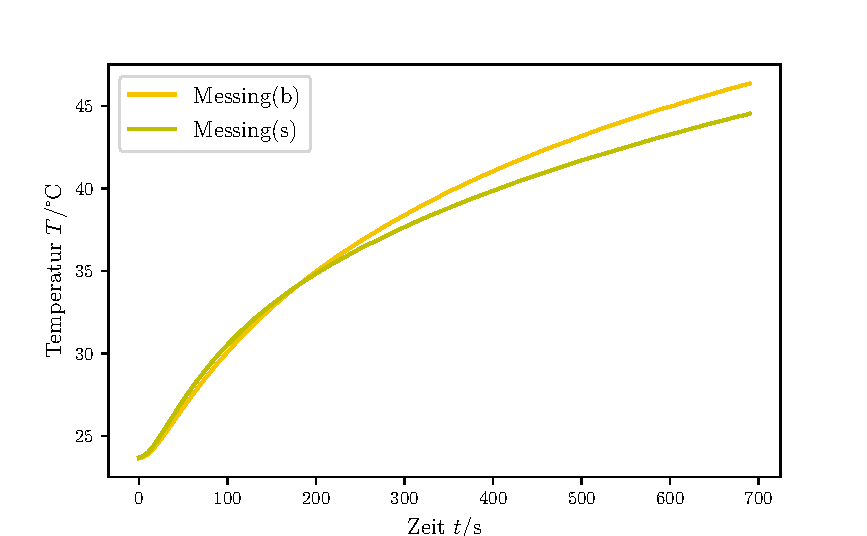
\includegraphics[max width=1.1\linewidth]{plots/plot_t1_t4.pdf}
        \caption{T1, T4.}
        \label{fig:plot_t1_t4}
    \end{subfigure}%
    \begin{subfigure}{.5\textwidth}
        \centering
        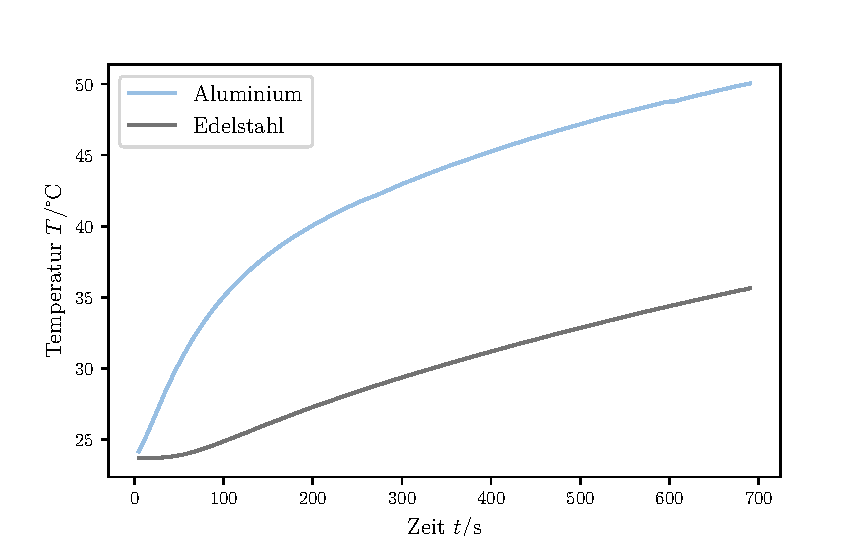
\includegraphics[max width=1.1\linewidth]{plots/plot_t5_t8.pdf}
        \caption{T5, T8}
        \label{fig:plot_t5_t8}
    \end{subfigure}
    \caption{Zeitliche Temperaturverläufe an den äußeren Sensoren}
    \label{fig:tempDiff_t1t4t5t8}
\end{figure}
Sowohl beide Messingproben als auch Aluminium weisen einen ähnlichen Funktionsgraphen auf, der augenscheinlich nur 
in horizontaler und vertikaler Skalierung variiert. 
In den etwa ersten 180 Sekunden steigt die Temperatur des schmalen Messingstabs minimal schneller an als der breite Stab. 
Danach hat der Graph des breiteren Stabs eine größere Steigung und beide Graphen steigen in gleichem Maße, um einen 
stetig wachsenden Temperaturunterschied versetzt, bis zur Endzeit.
Aluminium erreicht insgesamt die höchste Endtemperatur mit etwa $\SI{50}{\celsius}$. 
Im Gegensatz dazu steht Edelstahl: Nach einer kurzen anfänglichen Phase, in der die Temperatur kaum steigt, wächst der 
Graph nahezu linear an, was sich merklich von den Graphen unterscheidet. 
Diese besitzen vielmehr die geschwungene Form einer Wurzel- oder Logarithmus-Funktion. 

Um die Wärmeleitung besser zu untersuchen, sind hier die Endtemperaturen nach annähernd $\SI{700}{\second}$ aufgeführt:
\begin{table}
    \centering
    \caption{Äußere Temperatur nach $\SI{690}{\second}$ in $\SI{}{\celsius}$.}
    \label{tab:temp_aussen}
    \begin{tabular}{S[table-format=3.1, round-mode=places, round-precision=1] S[table-format=2.2] S[table-format=2.2] S[table-format=2.2] S[table-format=2.2]}
        \toprule
        {$t$} & {Messing(b)} & {Messing(s)} & {Aluminium} & {Edelstahl} \\
        \midrule
        690.0 & 46.36 &	44.53 &	50.04 &	35.64  \\
        \bottomrule
    \end{tabular}
\end{table}
Wie bereits erähnt hat Aluminium die höchste Endtemperatur erreicht, danach folgen der breite, der schmale Messingstab 
und Edelstahl in ebendieser Reihenfolge. 
Dementsprechend staffelt sich ebenfalls das zugehörige Maß der Wärmeleitung der einzelnen Proben. 

Nun soll für fünf verschiedene Messzeiten der Wärmestrom bestimmt werden, die sich über die Formel 
\begin{equation}
    \frac{\increment \symup{Q}}{\increment \symup{t}} = -\kappa A \frac{\increment \symup{T}}{\increment \symup{x}}
\end{equation}
berechnen lässt (vgl. dazu die Gleichung \eqref{eqn:waermestrom}). 
Hierbei gelten für Aluminium und Edelstahl ebenso die Maße der breiten Querschnittsfläche 
\begin{align*}
\symup{A}_{breit} = \SI{1.2}{\centi\m} \times \SI{0.4}{\centi\m} = \SI{0.48}{\square\centi\m},
\end{align*}
wohingegen der schmale Messingstab die Maße
\begin{align*}
\symup{A}_{schmal} = \SI{0.7}{\centi\m} \times \SI{0.4}{\centi\m} = \SI{0.28}{\square\centi\m} 
\end{align*}
erfüllt.
Bewusste Messwerte zu fünf verschiedenen Messzeiten und die sich daraus ergebenden Temperaturdifferenzen 
sind in Tabelle \ref{tab:temp_5_messwerte} und \ref{tab:tempdiff_5_messwerte} dargestellt. 
\begin{table}
    \centering
    \caption{Temperatur fünf verschiedener Messzeiten in $\si{\celsius}$.}
    \label{tab:temp_5_messwerte}
    \begin{tabular}{S[table-format=3, round-mode=places, round-precision=1] S[table-format=2.2] S[table-format=2.2] S[table-format=2.2] S[table-format=2.2] S[table-format=2.2] S[table-format=2.2] S[table-format=2.2] S[table-format=2.2]}
        \toprule
        & \multicolumn{2}{c}{Messing(breit)} & \multicolumn{2}{c}{Messing(schmal)} & \multicolumn{2}{c}{Aluminium} & \multicolumn{2}{c}{Edelstahl} \\
        \cmidrule(lr){2-3}\cmidrule(lr){4-5}\cmidrule(lr){6-7}\cmidrule(lr){8-9}
        {$t[\si{\s}]$} & {$T_{1, \text{fern}}$} & {$T_{2, \text{nah}}$} & {$T_{3, \text{nah}}$} & {$T_{4, \text{fern}}$} & {$T_{5, \text{fern}}$} & {$T_{6, \text{nah}}$} & {$T_{7, \text{nah}}$} & {$T_{8, \text{fern}}$} \\
        \midrule
        60  & 27.45 &	31.68 &	32.57 &	27.94 &  31.50 & 34.49 & 29.59 & 24.03 \\
        150 & 32.77 &	36.49 &	36.83 &	32.97 &  38.00 & 40.03 & 34.40 & 26.11 \\
        295 & 38.24 &	41.41 &	40.97 &	37.54 &  42.83 & 44.47 & 38.19 & 29.27 \\
        475 & 42.69 &	45.63 &	44.63 &	41.26 &  46.73 & 48.27 & 41.70 & 32.46 \\
        640 & 45.61 &	48.52 &	47.26 &	43.85 &  49.33 & 50.89 & 44.27 & 34.95 \\
        \bottomrule
    \end{tabular}
\end{table}

\begin{table}
    \centering
    \caption{Temperaturunterschied nah zu fern in $\si{\kelvin}$.}
    \label{tab:tempdiff_5_messwerte}
    \begin{tabular}{S[table-format=3, round-mode=places, round-precision=1] S[table-format=1.2, round-mode=places, round-precision=2] S[table-format=1.2, round-mode=places, round-precision=2] S[table-format=1.2, round-mode=places, round-precision=2] S[table-format=1.2, round-mode=places, round-precision=2]}
        \toprule
        {$t[\si{\s}]$} & {$\increment T_{Messing(breit)}$} & {$\increment T_{Messing(schmal)}$} & {$\increment T_{Aluminium}$} & {$\increment T_{Edelstahl}$} \\
        \midrule
        60  & 4.23   & 4.6299 & 2.99 &	5.559 \\
        150 & 3.7199 & 3.8599 & 2.03 &	8.29 \\
        295 & 3.1699 & 3.4299 & 1.64 &	8.91 \\
        475 & 2.94   & 3.370  & 1.54 &	9.24 \\
        640 & 2.91   & 3.4099 & 1.56 &	9.32 \\
        \bottomrule
    \end{tabular}
\end{table}

Die Werte für die materialabhängige Wärmeleitfähigkeit werden der Tabelle \ref{tab:Literaturwerte} mit den im Vorraus 
recherchierten Literaturwerten entnommen, 
der Abstand zweier Temperatursensoren ist gemäß der Messung $\increment x = \SI{3.0}{\centi\meter}$. 
Daraus ergeben sich die in Tabelle \ref{tab:Warmestrom} dargestellten Zahlenwerte für den Wärmestrom.
\begin{table}
    \centering
    \caption{Wärmestrom $\frac{\increment \symup{Q}}{\increment \symup{t}}$ in $\si{\joule\per\second}$.}
    \label{tab:Warmestrom}
    \begin{tabular}{l | S[round-mode=places, round-precision=4] S[round-mode=places, round-precision=4] S[round-mode=places, round-precision=4] S[round-mode=places, round-precision=4] S[round-mode=places, round-precision=4]}
        \toprule
        {Stoff} & {$\SI{60}{\s}$} & {$\SI{150}{\s}$} & {$\SI{295}{\s}$} & {$\SI{475}{\s}$} & {$\SI{640}{\s}$} \\
        \midrule
        Messing(breit)      & 0.758016    & 0.6666  & 0.56806 & 0.52684   & 0.52147   \\
        Messing(schmal)     & 0.483989  & 0.40349 & 0.358549 & 0.352277 & 0.35645 \\
        Aluminium           & 1.05726    & 0.71780   & 0.57990   & 0.54454   & 0.5516   \\
        Edelstahl           & 0.4092   & 0.61014  & 0.6565119 & 0.68006   & 0.68595   \\
        \bottomrule
    \end{tabular}
\end{table}

Des Weiteren sollen die an den Sensoren T7 und T8 beziehungsweise T2 und T1 gemessenen Temperaturdifferenzen in einem 
Diagramm der Zeit $t$ aufgetragen werden, also die Temperaturunterschiede an zwei verschiedenen Orten desselben Stabs, 
hier Edelstahl und Messing.
\begin{figure}
    \centering
    \begin{subfigure}{.5\textwidth}
        \centering
        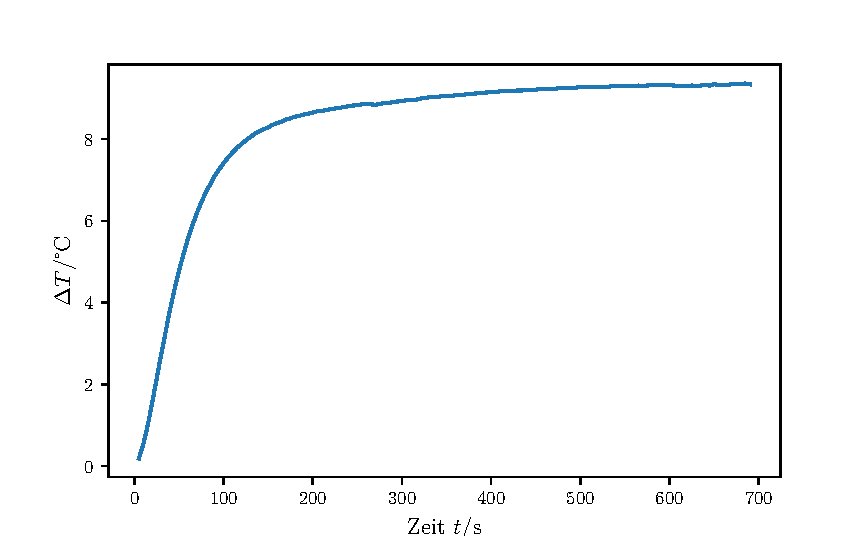
\includegraphics[max width=1.1\linewidth]{plots/plot_tempDiff_steel.pdf}
        \caption{$T7 - T8$ (Edelstahl).}
        \label{fig:plot_tempDiff_t7t8}
    \end{subfigure}%
    \begin{subfigure}{.5\textwidth}
        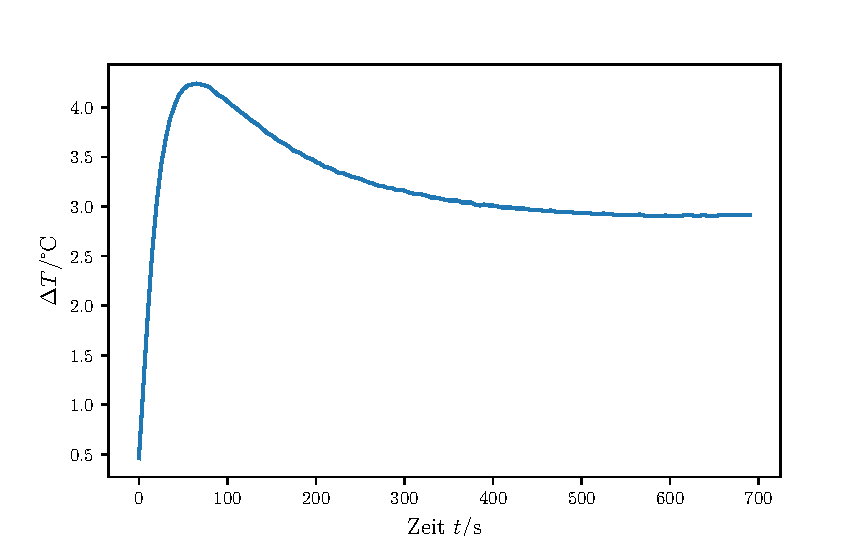
\includegraphics[max width=1.1\linewidth]{plots/plot_tempDiff_brass_wide.pdf}
        \caption{$T2 - T1$ (Messing).}
        \label{fig:plot_tempDiff_t2t1}
    \end{subfigure}
    \caption{Temperaturdifferenzen}
    \label{fig:tempDiff_t1t4t5t8}
\end{figure}

Beide Graphen haben anfänglich einen starken Anstieg, bei dem Edelstahl einen etwa doppelt so großen Wert erreicht wie Messing. 
Danach flacht die Differenz des Messings exponentiell ab, wohingegen die des Edelstahls sich asymptotisch einem Maximalwert nähert. 
Das zu Beginn starke Ansteigen indiziert das Anlegen einer dem Metall gegenüber höheren Temperatur, die zuerst am nahen 
Sensor registriert wird und erst mit einiger Zeitverzögerung an der weiter entfernten Messstelle. 
Die Temperaturdifferenz des Edelstahls steigt weiter an, das Temperaturgefälle nimmt also zu.
Dahingegen findet beim Messing ein schleichender Ausgleich der hohen Differenz statt, die Wärme verteilt sich gleichmäßiger auf dem Stab.  

\begin{table}
    \centering
    \caption{Messreihe 2 - Dynamische Methode}
    \label{tab:data2}
    \begin{tabular}{S[table-format=3.1, round-mode=places, round-precision=1] S[table-format=2.2] S[table-format=2.2] S[table-format=2.2] S[table-format=2.2] S[table-format=2.2] S[table-format=2.2] S[table-format=2.2] S[table-format=2.2]}
        \toprule
        & \multicolumn{2}{c}{Messing(breit)} & \multicolumn{2}{c}{Messing(schmal)} & \multicolumn{2}{c}{Aluminium} & \multicolumn{2}{c}{Edelstahl} \\
        \cmidrule(lr){2-3}\cmidrule(lr){4-5}\cmidrule(lr){6-7}\cmidrule(lr){8-9}
        {$t$} & {$T_{1, \text{fern}}$} & {$T_{2, \text{nah}}$} & {$T_{3, \text{nah}}$} & {$T_{4, \text{fern}}$} & {$T_{5, \text{fern}}$} & {$T_{6, \text{nah}}$} & {$T_{7, \text{nah}}$} & {$T_{8, \text{fern}}$} \\
        \midrule
        0.000 & 33.08 &	36.21 &	36.46 &	32.47 &	34.62 &	37.16 &	33.62 &	29.54 \\
        0.500 & 33.10 &	36.25 &	36.48 &	32.50 &	34.66 &	37.19 &	33.65 &	29.55 \\
        1.000 & 33.12 &	36.27 &	36.51 &	32.52 &	34.69 &	37.25 &	33.68 &	29.54 \\
        $\vdots$ & $\vdots$ & $\vdots$ & $\vdots$ & $\vdots$ & $\vdots$ & $\vdots$ & $\vdots$ & $\vdots$ \\
        882.00 & 65.16 & 65.67 & 62.65 & 61.61 & 67.34 & 65.75 & 62.62 & 50.17 \\
        \bottomrule
    \end{tabular}
\end{table}

Bei der dynamischen Messung sollen nach dem ersten Durchgang beide Temperaturverläufe der Messstellen am breiten Messingstab 
aufgetragen und die Amplituden $A_1$ und $A_2$ bei den jeweiligen Sensoren bestimmt werden. 
Dafür wurde eine Ausgleichskurve durch die Minima gezogen und die Differenz der Maxima zu dem entsprechenden Funktionswert
der Ausgleichskurve berechnet (vgl. Tabelle \ref{tab:amps_brass}). 
\begin{figure}
    \centering
    \begin{subfigure}{.5\textwidth}
        \centering
        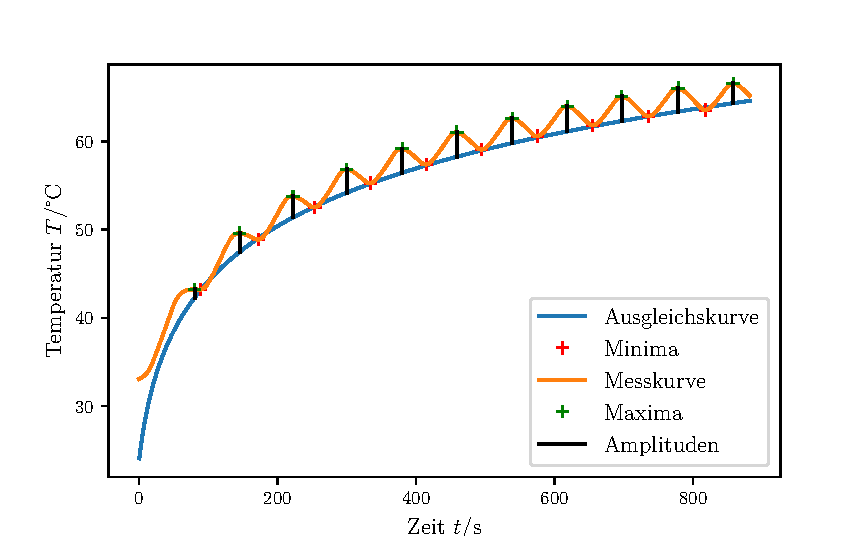
\includegraphics[max width=1.1\linewidth]{plots/amplitudes_brass_wide_far(t1).pdf}
        \caption{T1, fern.}
        \label{fig:plot_amps_t1}
    \end{subfigure}%
    \begin{subfigure}{.5\textwidth}
        \centering
        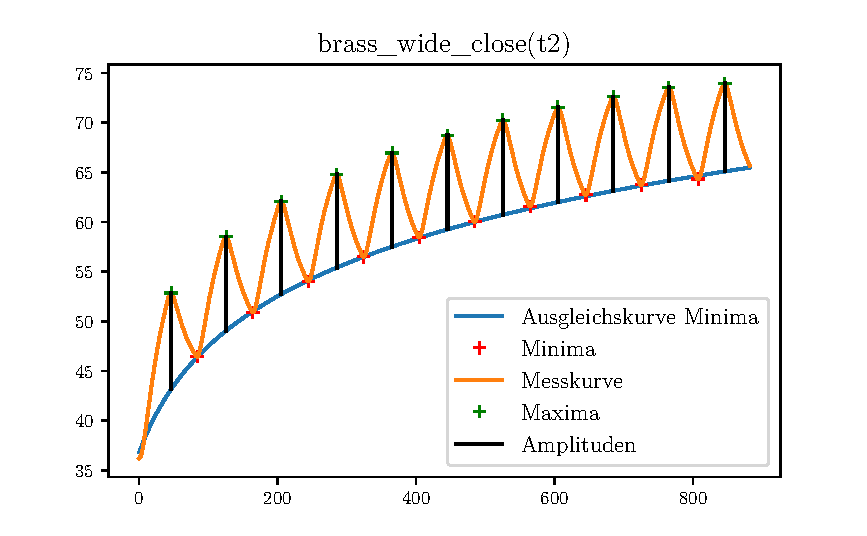
\includegraphics[max width=1.1\linewidth]{plots/amplitudes_brass_wide_close(t2).pdf}
        \caption{T2, nah.}
        \label{fig:plot_amps_t2}
    \end{subfigure}
    \caption{Messwertanalyse zu Messing(breit).}
    \label{fig:plots_amps_t1_t2}
\end{figure}
\begin{table}
    \centering
    \caption{Amplituden von Messing, nah und fern, in $\si{\kelvin}$.}
    \label{tab:amps_brass}
    \begin{tabular}{S[table-format=2.1] | S[table-format=3.1] S[table-format=1.2] @{${}$\pm${}$} S[table-format=1.2] | S[table-format=3.1] S[table-format=1.2] @{${}$\pm${}$} S[table-format=1.2]}
        \toprule
         & \multicolumn{3}{c}{$\symup{Messing}_\text{nah}$} & \multicolumn{3}{c}{$\symup{Messing}_\text{fern}$} \\
        \cmidrule(lr){2-4}\cmidrule(lr){5-7}
        {$\increment t[\si{\second}]$} &{$t[\si{\second}]$} & \multicolumn{2}{c}{$\increment T[{\si{\kelvin}]}$} & {$t[\si{\s}]$} & \multicolumn{2}{c}{$\increment T[{\si{\kelvin}]}$} \\
        \midrule
        34.0   &  46.5 &	9.64 & 0.23 &    80.5 & 0.89 & 0.20 \\	
        19.5   & 126.0 &	9.54 & 0.23 &   145.5 & 2.13 & 0.20 \\		
        17.0   & 205.5 &	9.49 & 0.23 &   222.5 & 2.53 & 0.20 \\		
        14.5   & 285.5 &	9.45 & 0.23 &   300.0 & 2.67 & 0.20 \\		
        14.5   & 365.5 &	9.42 & 0.23 &   380.0 & 2.71 & 0.20 \\		
        13.5   & 445.5 &	9.39 & 0.23 &   459.0 & 2.71 & 0.20 \\		
        13.5   & 525.5 &	9.37 & 0.23 &   539.0 & 2.70 & 0.20 \\		
        13.5   & 605.0 &	9.35 & 0.23 &   618.5 & 2.68 & 0.20 \\		
        12.0   & 685.0 &	9.34 & 0.23 &   697.0 & 2.65 & 0.20 \\		
        13.5   & 765.0 &	9.32 & 0.23 &   778.5 & 2.62 & 0.20 \\ 
        12.0   & 846.0 &	9.31 & 0.23 &   858.0 & 2.59 & 0.20	\\
        \bottomrule
    \end{tabular}
\end{table}
Die Maxima der Temperaturkurve werden aus der Messtabelle abgelesen, da hinreichend viele Werte gegeben sind.
Zur Berechnung der Ausgleichskurve durch die Minima wird der Ansatz $\symup{f(x)}=\symup{c}*np.log(x-\symup{a})+\symup{b}$
mit den Parametern $\symup{a, b, c}$ verwendet. 
Mithilfe der numerischen Methode der kleinsten Quadrate, die durch ein entsprechendes Computerprogramm durchgeführt wird,
werden diese Parameter dann bestimmt. 
So ergibt sich für die Paramter von T1 $\symup{(a,b,c)}=(-14.69279466, -2.94742813, 9.93498876)$ und für T2 
$\symup{(a,b,c)}=(-50.49563487, -1.97913302, 9.86737879)$.
Dasselbe wird nun für die Maxima gemacht.
Die Differenz der abgelesenen Werte und der an der entsprechenden Stelle ausgewerteten Funktion wird berechnet. 
Mittels dieser Differenzen werden die Varianz $V(X)$ und somit die Standardabweichung $\sigma_x$ ermittelt (bei N Messwerten). 
\begin{equation*}
V(X)= \frac{1}{N} \sum_{i=0}^N \increment x_i ^2 

\sigma_x = \sqrt{V(X)} 
\end{equation*}
Nun wird nach Gleichung \eqref{eqn:kappa} die Wärmeleitfähigkeit berechnet. 
% \begin{table}
%     \centering
%     \caption{Messing.}
%     \label{tab:unc_brass}
%     \begin{tabular}{S S S S S S | S S S S S S}
%         \toprule
%         \multicolumn{8}{c}{$\symup{Messing}_\text{nah}$} & \multicolumn{8}{c}{$\symup{Messing}_\text{fern}$} \\
%         \cmidrule(lr){1-4}\cmidrule(lr){5-8}\cmidrule(lr){9-12}\cmidrule(lr){13-16}
%         {$\increment t_{min} [\si{\second}]$} & {T2 min} & {$\increment T_{min}$} & {$\increment t_{max} [\si{\second}]$} & {T2 max} & {$\increment T_{max}$} & 
%         {$\increment t_{min} [\si{\second}]$} & {T1 min} & {$\increment T_{min}$} & {$\increment t_{max} [\si{\second}]$} & {T1 max} & {$\increment T_{max}$}\\
%         \midrule
%         %hier entsprechende Zwischenwerte einfügen
%         \bottomrule
%     \end{tabular}
% \end{table}
% \begin{table}
%     \centering
%     \caption{Wärmeleitfähigkeit $\kappa$ für Messing pro Amplitude.}
%     \label{tab:kappa_brass}
%     \begin{tabular}{S S}
%         \toprule
%         {$i$} & {$\kappa_i$} \\
%         \midrule
%         1 &    \\  %hier berechnete werte für kappa einfügen
%         2 &    \\ 
%         3 &    \\ 
%         4 &    \\ 
%         5 &    \\ 
%         6 &    \\ 
%         7 &    \\ 
%         8 &    \\ 
%           &    \\ 
%     \end{tabular}
% \end{table}
Der Mittelwert der verschiedenen Werte für $\kappa$ berechnet sich durch 
\begin{equation}
\bar{x} = \frac{1}{N} \sum_{i=1}^N x_i .
\label{eqn:average}
\end{equation}
Für die Messgröße $x$ erhält man dann $x = \bar{x} \pm \sigma_x$.
Für die Wärmeleitfähigkeit des Messings ergibt sich an dieser Stelle somit $\kappa = \SI{75 \pm 22}{\watt\per\meter\per\kelvin} $.

Dasselbe Vorgehen soll bei Aluminium durchgeführt werden:
\begin{figure}
    \centering
    \begin{subfigure}{.5\textwidth}
        \centering
        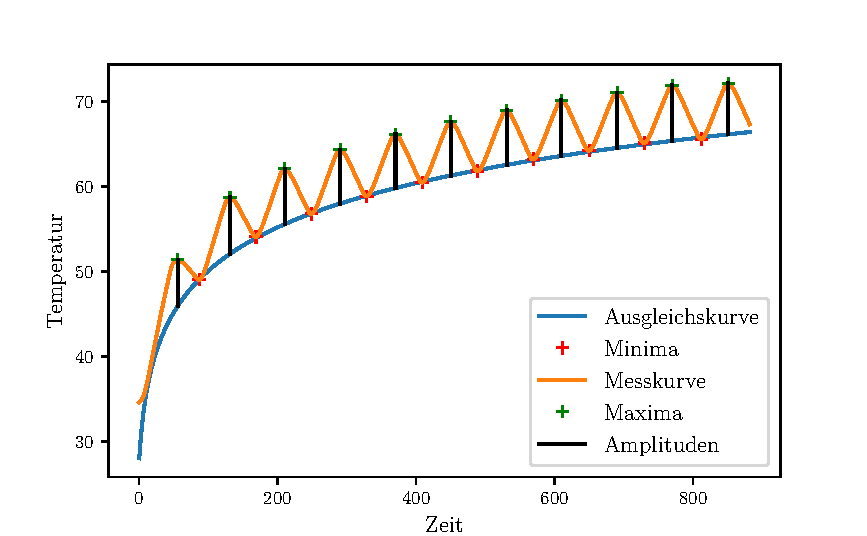
\includegraphics[max width=1.1\linewidth]{plots/amplitudes_aluminum_far(t5).pdf}
        \caption{T5, fern.}
        \label{fig:plot_amps_t5}
    \end{subfigure}%
    \begin{subfigure}{.5\textwidth}
        \centering
        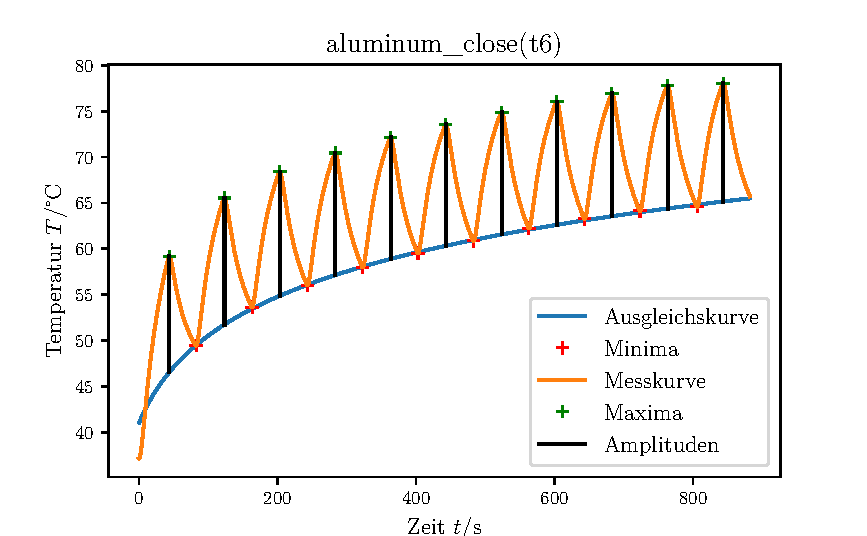
\includegraphics[max width=1.1\linewidth]{plots/amplitudes_aluminum_close(t6).pdf}
        \caption{T6, nah.}
        \label{fig:plot_amps_t6}
    \end{subfigure}
    \caption{Messwertanalyse zu Aluminium.}
    \label{fig:plots_amps_t5_t6}
\end{figure}
\begin{table}
    \centering
    \caption{Amplituden von Aluminium, nah und fern, in $\si{\kelvin}$.}
    \label{tab:amps_alu}
    \begin{tabular}{S[table-format=2.1] | S[table-format=3.1] S[table-format=2.2] @{${}$\pm${}$} S[table-format=1.2] | S[table-format=3.1] S[table-format=1.2] @{${}$\pm${}$} S[table-format=1.2]}
        \toprule
         & \multicolumn{3}{c}{$\symup{Aluminium}_\text{nah}$} & \multicolumn{3}{c}{$\symup{Aluminium}_\text{fern}$} \\
        \cmidrule(lr){2-4}\cmidrule(lr){5-7}
        {$\increment t[\si{\second}]$} &{$t[\si{\second}]$} & \multicolumn{2}{c}{$\increment T[{\si{\kelvin}]}$} & {$t[\si{\s}]$} & \multicolumn{2}{c}{$\increment T[{\si{\kelvin}]}$} \\
        \midrule
        12.0  &  44.0 &	12.68 & 0.24 &    56.0 &	5.50 & 0.21 \\
        8.0   & 123.5 &	13.44 & 0.24 &   131.5 &	6.41 & 0.21 \\		
        7.0   & 203.5 &	13.54 & 0.24 &   210.5 &	6.53 & 0.21 \\		
        7.0   & 283.5 &	13.51 & 0.24 &   290.5 &	6.53 & 0.21 \\		
        7.0   & 363.5 &	13.46 & 0.24 &   370.5 &	6.50 & 0.21 \\		
        7.0   & 443.0 &	13.39 & 0.24 &   450.0 &	6.45 & 0.21 \\		
        7.0   & 524.0 &	13.32 & 0.24 &   531.0 &	6.41 & 0.21 \\		
        6.5   & 603.5 &	13.26 & 0.24 &   610.0 &	6.37 & 0.21 \\		
        7.5   & 683.0 &	13.20 & 0.24 &   690.5 &	6.33 & 0.21 \\		
        6.5   & 763.5 &	13.14 & 0.24 &   770.0 &	6.29 & 0.21 \\
        7.5   & 843.5 &	13.09 & 0.24 &   851.0 &	6.25 & 0.21 \\
        \bottomrule
    \end{tabular}
\end{table}

T5, Minima: $\symup{(a,b,c)}=([-5.43820767, 14.36801819, 7.66920384])$ \\
T6, Minima: $\symup{(a,b,c)}=([-43.92552164, 10.56412431, 8.04223001])$
% T5, Maxima: $\symup{(a,b,c)}=()$ %Parameter für T5 und T6 einfügen
% T6, Maxima: $\symup{(a,b,c)}=()$

% \begin{table}
%     \centering
%     \caption{Aluminium.}
%     \label{tab:unc_alu}
%     \begin{tabular}{S S S S S S S S | S S S S S S S S}
%         \toprule
%         \multicolumn{8}{c}{$\symup{Messing}_\text{nah}$} & \multicolumn{8}{c}{$\symup{Messing}_\text{fern}$} \\
%         \cmidrule(lr){1-4}\cmidrule(lr){5-8}\cmidrule(lr){9-12}\cmidrule(lr){13-16}
%         {$\increment t_min [\si{\second}]$} & {abgelesene Minima T6} & {$\symup{f_t6(t_min)}$} & {$\increment T_min$} & {$\increment t_max [\si{\second}]$} & {abgelesene Maxima T6} & {$\symup{f_t6(t_max)}$} & {$\increment T_max$} & 
%         {$\increment t_min [\si{\second}]$} & {abgelesene Minima T5} & {$\symup{f_t5(t_min)}$} & {$\increment T_min$} & {$\increment t_max [\si{\second}]$} & {abgelesene Maxima T5} & {$\symup{f_t5(t_max)}$} & {$\increment T_max$}\\
%         \midrule
%         %hier entsprechende Zwischenwerte einfügen
%         \bottomrule
%     \end{tabular}
% \end{table}
% \begin{table}
%     \centering
%     \caption{Wärmeleitfähigkeit $\kappa$ für Aluminium pro Amplitude.}
%     \label{tab:kappa_alu}
%     \begin{tabular}{S S}
%         \toprule
%         {$i$} & {$\kappa_i$} \\
%         \midrule
%         1 &   \\%hier berechnete werte für kappa einfügen
%         2 &   \\
%         3 &   \\
%         4 &   \\
%         5 &   \\
%         6 &   \\
%         7 &   \\
%         8 &   \\
%           &   \\
%     \end{tabular}
% \end{table}
Für die Wärmeleitfähigkeit des Aluminiums ergibt sich an dieser Stelle somit $\kappa = \SI{206 \pm 33}{\watt\per\meter\per\kelvin}  $

Für die letzte Messreihe soll dieses Verfahren nochmal für Edelstahl durchgeführt werden:
\begin{figure}
    \centering
    \begin{subfigure}{.5\textwidth}
        \centering
        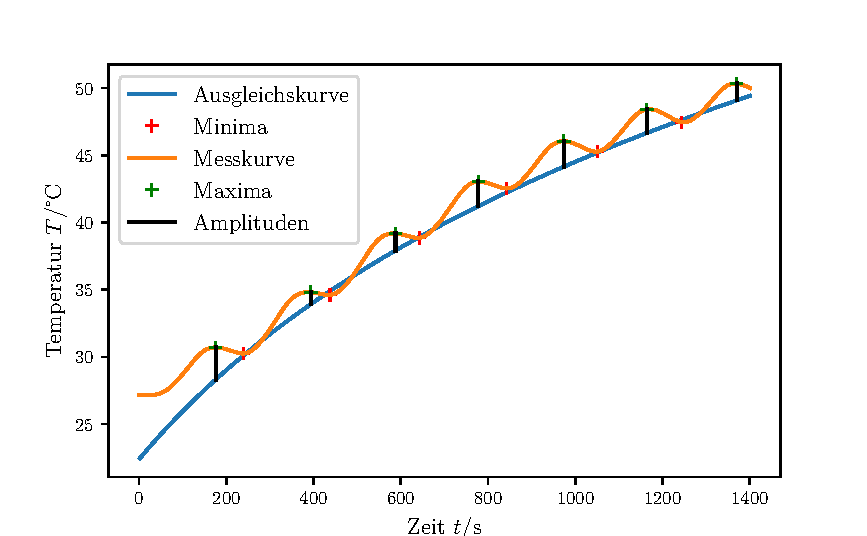
\includegraphics[max width=1.1\linewidth]{plots/amplitudes_steel_far(t8).pdf}
        \caption{T8, fern.}
        \label{fig:plot_amps_t8}
    \end{subfigure}%
    \begin{subfigure}{.5\textwidth}
        \centering
        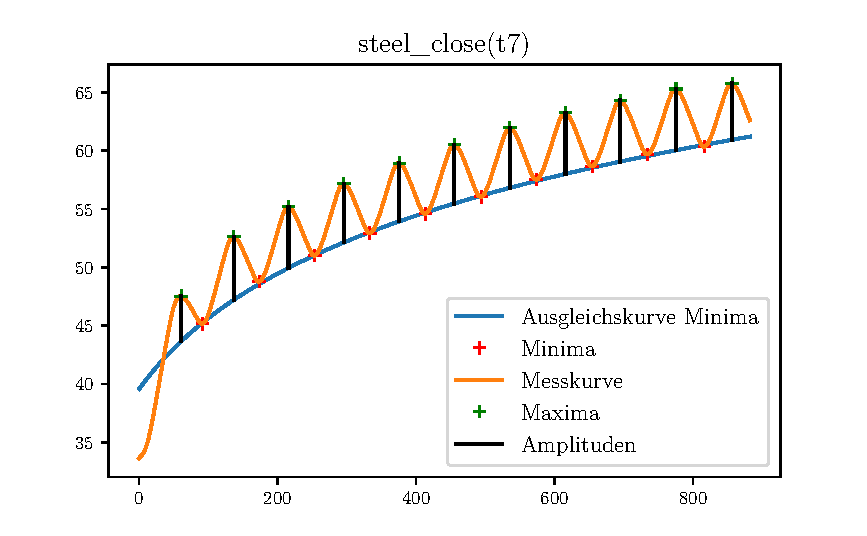
\includegraphics[max width=1.1\linewidth]{plots/amplitudes_steel_close(t7).pdf}
        \caption{T7, nah.}
        \label{fig:plot_amps_t7}
    \end{subfigure}
    \caption{Messwertanalyse zu Aluminium.}
    \label{fig:plots_amps_t7_t8}
\end{figure}
\begin{table}
    \centering
    \caption{Amplituden von Edelstahl, nah und fern, in $\si{\kelvin}$.}
    \label{tab:amps_steel}
    \begin{tabular}{S[table-format=2.1] | S[table-format=3.1] S[table-format=2.1] @{${}$\pm${}$} S[table-format=1.1] | S[table-format=3.1] S[table-format=1.1] @{${}$\pm${}$} S[table-format=1.1]}
        \toprule
         & \multicolumn{3}{c}{$\symup{Edelstahl}_\text{nah}$} & \multicolumn{3}{c}{$\symup{Edelstahl}_\text{fern}$} \\
        \cmidrule(lr){2-4}\cmidrule(lr){5-7}
        {$\increment t[\si{\second}]$} &{$t[\si{\second}]$} & \multicolumn{2}{c}{$\increment T[{\si{\kelvin}]}$} & {$t[\si{\s}]$} & \multicolumn{2}{c}{$\increment T[{\si{\kelvin}]}$} \\
        \midrule
        66.0   & 110.0	& 17.1 & 0.4 &   176.0  &	2.1 & 0.5 \\
        84.0   & 310.0	& 15.2 & 0.4 &   394.0  &	1.6 & 0.5 \\		
        78.0   & 510.0	& 14.8 & 0.4 &   588.0  &	1.4 & 0.5 \\		
        64.0   & 714.0	& 14.6 & 0.4 &   778.0  &	1.4 & 0.5 \\		
        64.0   & 910.0	& 14.6 & 0.4 &   974.0  &	1.5 & 0.5 \\		
        54.0   & 1110.0	& 14.6 & 0.4 &   1164.0 &	1.6 & 0.5 \\		
        60.0   & 1310.0	& 14.6 & 0.4 &   1370.0 &	1.7 & 0.5 \\		
        \bottomrule
    \end{tabular}
\end{table}

T7, Minima: $\symup{(a,b,c)}=([-78.40062517, -52.64024484, 14.83964357])$ \\
T8, Minima: $\symup{(a,b,c)}=([-547.28040531, -111.97054179, 21.30691517])$

% \begin{table}
%     \centering
%     \caption{Edelstahl.}
%     \label{tab:unc_steel}
%     \begin{tabular}{S S S S S S S S | S S S S S S S S}
%         \toprule
%         \multicolumn{8}{c}{$\symup{Edelstahl}_\text{nah}$} & \multicolumn{8}{c}{$\symup{Edelstahl}_\text{fern}$} \\
%         \cmidrule(lr){1-4}\cmidrule(lr){5-8}\cmidrule(lr){9-12}\cmidrule(lr){13-16}
%         {$\increment t_min [\si{\second}]$} & {abgelesene Minima T7} & {$\symup{f_t7(t_min)}$} & {$\increment T_min$} & {$\increment t_max [\si{\second}]$} & {abgelesene Maxima T7} & {$\symup{f_t7(t_max)}$} & {$\increment T_max$} & 
%         {$\increment t_min [\si{\second}]$} & {abgelesene Minima T8} & {$\symup{f_t8(t_min)}$} & {$\increment T_min$} & {$\increment t_max [\si{\second}]$} & {abgelesene Maxima T8} & {$\symup{f_t8(t_max)}$} & {$\increment T_max$}\\
%         \midrule
%         %hier entsprechende Zwischenwerte einfügen
%         \bottomrule
%     \end{tabular}
% \end{table}
% \begin{table}
%     \centering
%     \caption{Wärmeleitfähigkeit $\kappa$ für Edelstahl pro Amplitude.}
%     \label{tab:kappa_steel}
%     \begin{tabular}{S S}
%         \toprule
%         {$i$} & {$\kappa_i$} \\
%         \midrule
%         1 &   \\%hier berechnete werte für kappa einfügen
%         2 &   \\
%         3 &   \\
%         4 &   \\
%         5 &   \\
%         6 &   \\
%         7 &   \\
%         8 &   \\
%           &   \\
%     \end{tabular}
% \end{table}
Für die Wärmeleitfähigkeit des Edelstahls ergibt sich an dieser Stelle somit $\kappa = \SI{11.0 \pm 1.7}{\watt\per\meter\per\kelvin}$

\section{Diskussion}
\label{sec:Diskussion}

\subsection{Anregung durch eine Rechteckspannung}

Der theoretisch zu erwartende Wert für die Zeitkonstante ist $\tau _\text{theo}=\SI{1.405(56)}{\milli\second}$, der aus dem 
ersten Teil des Experiments ermittelte ${\tau _\text{exp}=\SI{0.82(1)}{\milli\second}}$. 
Da der experimentelle Wert deutlich außerhalb des Fehlerintervalls von $\tau _\text{theo}$ liegt, kann an dieser Stelle 
nicht von einer statistischen Abweichung ausgegangen werden. 
Der Fehler kann auch nicht an nicht berücksichtigten Innenwiderständen der Geräte oder an ohmschen Verlusten der Kabel 
liegen. 
Wahrscheinlicher ist ein systematischer Messfehler, der sich im Nachhinein nur schwerlich zu finden lässt. 
Möglichkeiten könnten überdrehte -- und deshalb keine richtig skalierenden -- Knöpfe am Oszilloskop sein, sodass alle 
abgelesenen Spannungswerte um einen Faktor verschieden von der tatsächlich angelegten Spannung sind. 

\subsection{Integrieren der Generatorspannung}

Bei allen drei Spannungen kann sehr gut die Phasenverschiebung um $\sfrac{\pi}{2}$ beobachtet werden, die wenn überhaupt 
nur minimal kleiner ist. 
Dies ist konsistent mit der Theorie, da nur für eine unendlich große Frequenz eine solche Phasendifferenz bewerkstelligt 
werden kann. Eine im mathematischen Sinne unendlich große Frequenz ist selbstredend in der Praxis nur näherungsweise zu 
realisieren. 

Bereits bei der Durchführung fällt auf, dass die Skala der Kondensatorspannung stark vergrößert werden muss, um Amplituden 
vergleichbarer Größenordnung auf dem Oszilloskop beobachten zu können. 
Dies rührt daher, dass bei hoher Frequenz ein vergleichsweise sehr kleiner Anteil der Spannung beim Kondensator ankommt, 
wie in der Theorie ausführlich erklärt wird. 

\begin{figure}
\centering
\begin{subfigure}{0.48\textwidth}
    \centering
    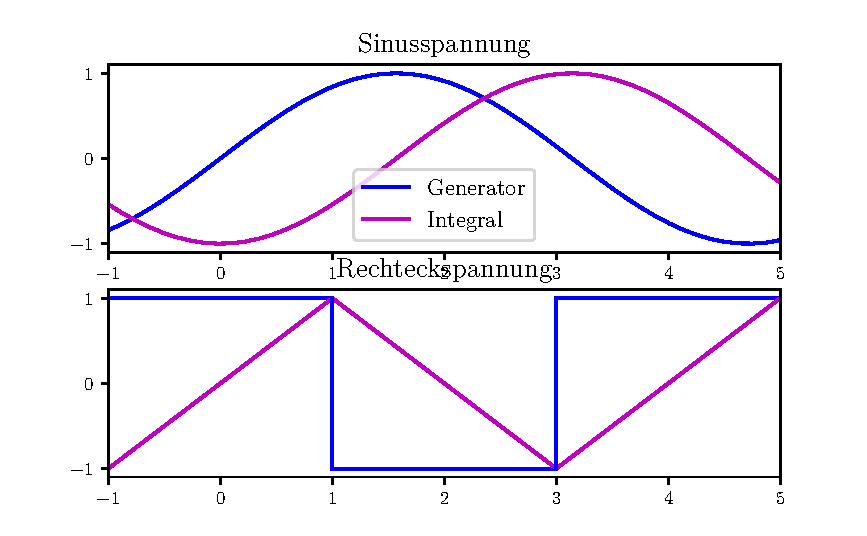
\includegraphics[height=5cm]{plots/erwart_int1.pdf}
    \label{fig:erw1}
\end{subfigure}
\begin{subfigure}{0.48\textwidth}
    \centering
    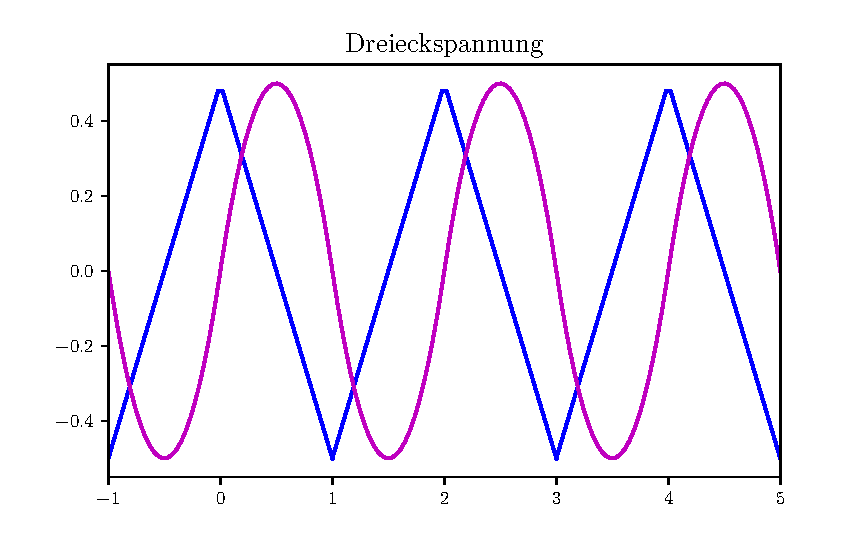
\includegraphics[height=5cm]{plots/erwart_int2.pdf}
    \label{fig:erw2}
\end{subfigure}
\caption{Die Spannungskurven und ihre zugehörigen Integrale.}
\label{fig:int}
\end{figure}

Um die Bilder vom Oszilloskop gut vergleichen zu können, sind in \ref{fig:int}  
die jeweiligen Spannungsarten mit zugehörigen Funktionsgraphen abgebildet, deren Ableitung die Spannungskurve ergibt. 
Der Übersicht halber wird an dieser Stelle auf eine explizite Darstellung der Funktionsdefinitionen von Dreiecks- und Rechteckskurven 
und deren Integrationen verzichtet. Sie bestehen aus trivialen linearen stückweise stetigen beziehungsweise differenzierbaren 
Funktionen. 

Wie durch einen Vergleich der Abbildungen klar ersichtlich ist, entsprechen die theoretischen Überlegungen bezüglich der 
integrierenden Eigenschaft eines RC-Kreises den experimentellen Beobachtungen. 
\newpage
\section*{Anhang: Messdaten}
\addcontentsline{toc}{section}{Anhang: Messdaten}% Fügt die section dem Inhaltsverzeichnis zu, nummeriert sie aber nicht

\begin{table}
    \centering
    \caption{Abgelesenen Messpunkte zur Auswertung für die Energieverteilung der Elektronen, Teil 1.}
    \label{tab:Energy1}
    \begin{tabular}{S[table-format=1.2] S[table-format=3.1] S[table-format=1.1] S[table-format=1.2] S[table-format=3.1] S[table-format=1.1]}
        \toprule
        $U_\text{A}\,/\,\si{\volt}$ & $I_\text{A}\,/\,\si{\nano\ampere}$ & $\Delta I_\text{A}\,/\,\si{\nano\ampere}$ &
        $U_\text{A}\,/\,\si{\volt}$ & $I_\text{A}\,/\,\si{\nano\ampere}$ & $\Delta I_\text{A}\,/\,\si{\nano\ampere}$ \\
        \midrule
        0.00 & 363.0 & 7.0 & 2.56 & 258.0 & 3.0 \\
        0.08 & 356.0 & 3.5 & 2.64 & 255.0 & 3.0 \\
        0.16 & 352.5 & 3.0 & 2.72 & 252.0 & 3.0 \\
        0.24 & 349.5 & 4.5 & 2.80 & 249.0 & 3.5 \\
        0.32 & 345.0 & 3.0 & 2.88 & 245.5 & 2.5 \\
        0.40 & 342.0 & 4.5 & 2.96 & 243.0 & 3.0 \\
        0.48 & 337.5 & 3.0 & 3.04 & 240.0 & 3.0 \\
        0.56 & 334.5 & 3.0 & 3.12 & 237.0 & 2.5 \\
        0.64 & 331.5 & 3.0 & 3.20 & 234.5 & 3.0 \\
        0.72 & 328.5 & 2.0 & 3.28 & 231.5 & 3.0 \\
        0.80 & 326.5 & 4.5 & 3.36 & 228.5 & 3.0 \\
        0.88 & 322.0 & 2.5 & 3.44 & 225.5 & 2.5 \\
        0.96 & 319.5 & 3.5 & 3.52 & 223.0 & 3.0 \\
        1.04 & 316.0 & 3.0 & 3.60 & 220.0 & 3.0 \\
        1.12 & 313.0 & 3.0 & 3.68 & 217.0 & 3.0 \\
        1.20 & 310.0 & 3.0 & 3.76 & 214.0 & 2.5 \\
        1.28 & 307.0 & 3.5 & 3.84 & 211.5 & 3.0 \\
        1.36 & 303.5 & 3.0 & 3.92 & 208.5 & 3.0 \\
        1.44 & 300.5 & 3.0 & 4.00 & 205.5 & 3.0 \\
        1.52 & 297.5 & 3.0 & 4.08 & 202.5 & 3.0 \\
        1.60 & 294.5 & 3.0 & 4.16 & 199.5 & 3.5 \\
        1.68 & 291.5 & 3.5 & 4.24 & 196.0 & 3.0 \\
        1.76 & 288.0 & 3.0 & 4.32 & 193.0 & 3.0 \\
        1.84 & 285.0 & 3.0 & 4.40 & 190.0 & 3.0 \\
        1.92 & 282.0 & 3.0 & 4.48 & 187.0 & 3.5 \\
        2.00 & 279.0 & 2.5 & 4.56 & 183.5 & 3.0 \\
        2.08 & 276.5 & 3.5 & 4.64 & 180.5 & 3.0 \\
        2.16 & 273.0 & 3.0 & 4.72 & 177.5 & 3.0 \\
        2.24 & 270.0 & 3.0 & 4.80 & 174.5 & 3.5 \\
        2.32 & 267.0 & 3.0 & 4.88 & 171.0 & 3.0 \\
        2.40 & 264.0 & 3.5 & 4.96 & 168.0 & 3.0 \\
        2.48 & 260.5 & 2.5 & 5.04 & 165.0 & 3.5 \\
        \bottomrule
    \end{tabular}
\end{table}
\begin{table}
    \centering
    \caption{Abgelesenen Messpunkte zur Auswertung für die Energieverteilung der Elektronen, Teil 2.}
    \label{tab:Energy2}
    \begin{tabular}{S[table-format=1.2] S[table-format=3.1] S[table-format=1.1] S[table-format=1.2] S[table-format=2.1] S[table-format=1.1]}
        \toprule
        $U_\text{A}\,/\,\si{\volt}$ & $I_\text{A}\,/\,\si{\nano\ampere}$ & $I_\text{A}\,/\,\si{\nano\ampere}$ &
        $U_\text{A}\,/\,\si{\volt}$ & $I_\text{A}\,/\,\si{\nano\ampere}$ & $I_\text{A}\,/\,\si{\nano\ampere}$ \\
        \midrule
        5.12 & 161.5 & 3.5 & 7.12 & 71.0 & 3.0 \\
        5.20 & 158.0 & 3.5 & 7.20 & 68.0 & 4.0 \\
        5.28 & 154.5 & 3.0 & 7.28 & 64.0 & 3.5 \\
        5.36 & 151.5 & 3.5 & 7.36 & 60.5 & 4.5 \\
        5.44 & 148.0 & 3.5 & 7.44 & 56.0 & 3.5 \\
        5.51 & 144.5 & 3.0 & 7.51 & 52.5 & 9.0 \\
        5.59 & 141.5 & 3.5 & 7.59 & 43.5 & 6.0 \\
        5.67 & 138.0 & 3.5 & 7.67 & 37.5 & 7.5 \\
        5.75 & 134.5 & 3.5 & 7.75 & 30.0 & 4.0 \\
        5.83 & 131.0 & 3.0 & 7.83 & 26.0 & 8.0 \\
        5.91 & 128.0 & 3.0 & 7.91 & 18.0 & 7.5 \\
        6.00 & 125.0 & 3.0 & 8.00 & 10.5 & 3.0 \\
        6.08 & 122.0 & 1.0 & 8.08 &  7.5 & 1.5 \\
        6.16 & 121.0 & 4.0 & 8.16 &  6.0 & 1.5 \\
        6.24 & 117.0 & 3.5 & 8.24 &  4.5 & 0.5 \\
        6.32 & 113.5 & 4.0 & 8.32 &  4.0 & 0.5 \\
        6.40 & 109.5 & 7.5 & 8.40 &  3.5 & 0.5 \\
        6.48 & 102.0 & 4.0 & 8.48 &  3.0 & 1.0 \\
        6.55 &  98.0 & 4.5 & 8.56 &  2.0 & 1.0 \\
        6.63 &  93.5 & 4.0 & 8.64 &  1.0 & 1.0 \\
        6.71 &  89.5 & 4.0 & 8.72 &  0.0 & 0.0 \\
        6.79 &  85.5 & 4.5 & 8.80 &  0.0 & 0.0 \\
        6.87 &  81.0 & 4.0 & 8.88 &  0.0 & 0.0 \\
        6.95 &  77.0 & 3.0 & 8.96 &  0.0 & 0.0 \\
        7.04 &  74.0 & 3.0 &      &      &     \\
        \bottomrule
    \end{tabular}
\end{table}
\begin{figure}
    \centering
    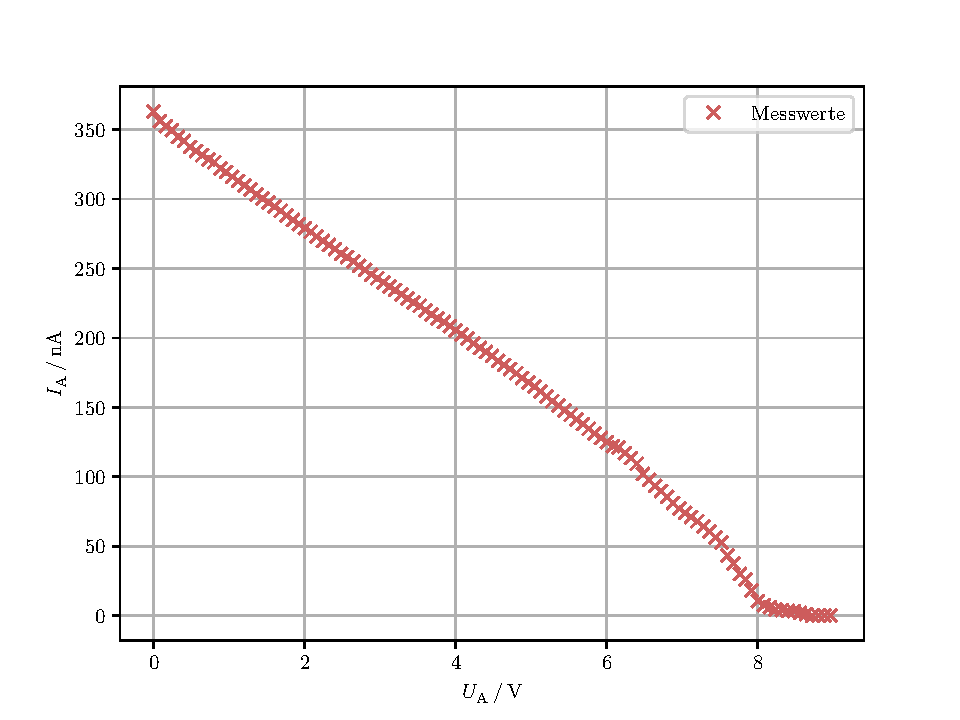
\includegraphics[width=\textwidth]{plots/Energie.pdf}
    \caption{Messwerte zur integralen Energieverteilung der Elektronen.}
    \label{fig:EnergieMess}
\end{figure}
\begin{figure}
    \centering
    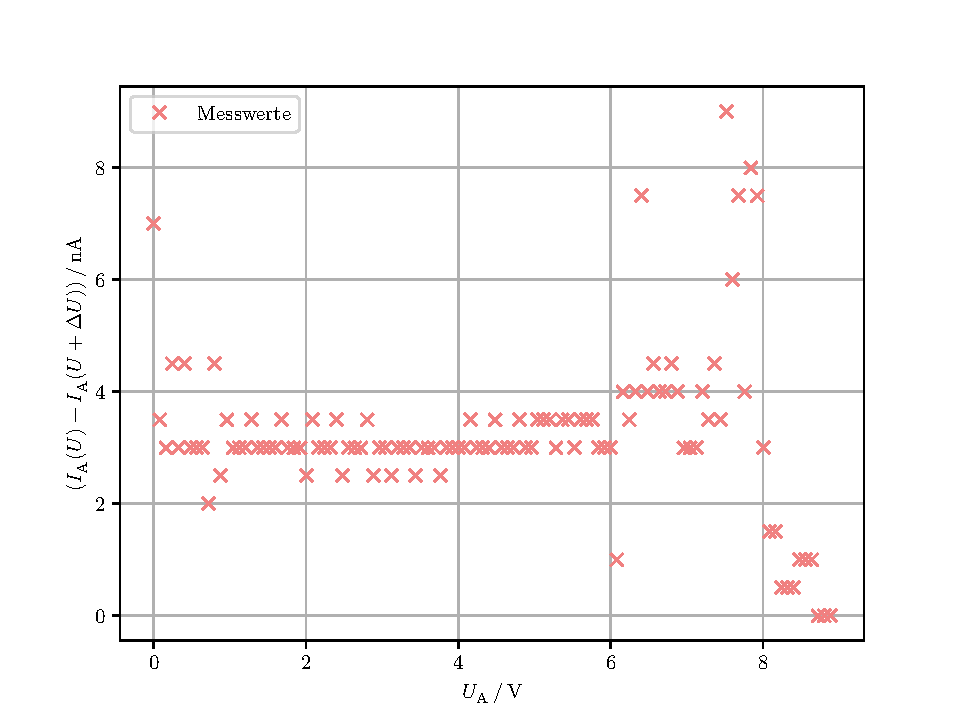
\includegraphics[width=\textwidth]{plots/EnergieDiff.pdf}
    \caption{Messwerte zur differentiellen Energieverteilung der Elektronen.}
    \label{fig:EnergieMess2}
\end{figure}

\printbibliography{}

\end{document}
